\documentclass{article}

\usepackage[utf8]{inputenc}
\usepackage[T1]{fontenc}
\usepackage[norsk,english]{babel} %norsk først så engelsk, så engelsk blir prioritert
\usepackage{graphicx}
\usepackage{amsmath}
\usepackage{listings}
\usepackage{hyperref}
\hypersetup{
    colorlinks,
    citecolor=black,
    filecolor=black,
    linkcolor=blue,
    urlcolor=blue
}

\setlength{\parindent}{0pt}

\setlength{\tabcolsep}{18pt}
\renewcommand{\arraystretch}{1.5}

%\newcounter{sectioncounter}
%\newenvironment{sections}[1][]{\addtocounter{sectioncounter}{1} \noindent {\bf \Large \arabic{sectioncounter} \ \ #1}\hspace{2mm}}{\vspace{4mm}}

\begin{document}

\addtocounter{page}{0}

\title{Project 1 \\
      \large For the course FYS3150}
\date{\today \\
    \vspace{1mm}
    \large Week 35-37}

\author{Erik Grammeltvedt, Erlend Tiberg North and Alexandra Jahr Kolstad}

\maketitle

%------------her starter skrivingen-----------------------------------------
\vspace{1cm}

\tableofcontents

%----------Abstract-------------------------------


\section{Abstract}

%\vspace{2mm}

We have developed an algorithm that computes...

Thomas algorithm, loss of numerical precision (FLOPS)


%--------------Introduction------------------------------
\vspace{1cm}

\section{Introduction}

{\large \bf les gjennom} \\

In this project we are going to solve Poisson's equation as a set of linear equations. Poisson's equation is a partial differential equation written in the file \textbf{Project1.pdf}. This equation can be rewritten as an ordinary differential equation

\begin{equation}
  - u''(x) = f(x)   \label{eq:u(x)diffeq}
\end{equation} \\

The functions we are operating with are

\begin{align}
  f(x) &= 100 e ^{-10 x}    \label{eq:f(x)eq} \\
  u(x) &= 1 - (1- e ^{-10}) x - e ^{- 10 x} \label{eq:u(x)eq}
\end{align} \\

These are also given in \textbf{Project1.pdf}. We are going to solve the ordinary differential equation by computing the decomposition and forward substitution and the backward substitution of the given matrices with the programming language \texttt{C++}. Our group is using the Armadillo package to more easily define and compute with matrices. We are also going to work with and try to understand dynamic memory allocation. The main exercise is grouped into smaller sub exercises ranging from \textbf{a)} to \textbf{e)}. \\

For the exercises \textbf{b)}, \textbf{c)}, \textbf{d)} and \textbf{e)} the main program is \texttt{thomas-algorithm.cpp}. For \textbf{b)}, \textbf{c)} and \textbf{e)} there are an additional program called \texttt{plot\_data.py} which plots the data. Only for exercise \textbf{c)} there is the program \texttt{timing.py} for comparing the time used in the different programs, and only for \textbf{d)} there is the program \texttt{error.py} which computes the error for the algorithm in \textbf{b)}. \\

\vspace{3mm}


%---------------Method------------------------------------
\vspace{1cm}

\section{Method}

  {\large \bf se gjennom} \\

\subsection{Exercise a)}

  In the exercise we are given the equation

  \begin{equation*}
    - \frac{v_{i+1} + v_{i-1} - 2 v_i}{h^2} = f_i \hspace{5mm} \textrm{for} ~  i = 1, 2, 3, ... , n
  \end{equation*}

  Rewrites the equation to
  \begin{align*}
    - (v_{i+1} + v_{i-1} - 2 v_i) &= h^2 f_i = \tilde{b}_i \\
    - v_{i+1} - v_{i-1} + 2 v_i &= \tilde{b}_i
  \end{align*}

  where in the exercise we are also given the correlation $\tilde{b}_i = h^2 f_i$, which is implemented here. \\

  Defines the equation for different values of the integer $i$ to get a set of equations. The exercise also gives the boundry conditions $v_0 = v_{n+1} = 0$.

  \begin{align*}
    i &= 1 : \hspace{5mm} - v_{1+1} - v_{1-1} + 2 v_1 = - v_2 - v_0 + 2 v_1 = - 0 + 2 v_1 - v_2 = \tilde{b}_1 \\
    i &= 2 : \hspace{5mm} - v_{2+1} - v_{2-1} + 2 v_2 = - v_3 - v_1 + 2 v_2 = - v_1 + 2 v_2 - v_3 = \tilde{b}_2 \\
    i &= 3 : \hspace{5mm} - v_{3+1} - v_{3-1} + 2 v_3 = - v_4 - v_2 + 2 v_3 = - v_2 + 2 v_3 - v_4 = \tilde{b}_3 \\
    \vdots \\
    i &= n : \hspace{5mm} - v_{n+1} - v_{n-1} + 2 v_n = - v_{n-1} + 2 v_n - 0 = \tilde{b}_n \\
  \end{align*}

  Equations can be rewritten as a matrix equation, which gives a matrix \textbf{A} with integers as elements, a vector $\vec{v} = [v_1, v_2, v_3, ... , v_n]$ and another vector $\vec{\tilde{b}} = [\tilde{b}_1, \tilde{b}_2, \tilde{b}_3, ... , \tilde{b}_n]$. This gives the matrix equation

  \begin{equation}
    \textbf{A} \vec{v} = \vec{\tilde{b}}  \label{eq:matrixeq}
  \end{equation} \\

  where $\vec{v}$ is the solution. The matrix and the vectors are given as

  \begin{equation*}
    \begin{bmatrix}
      2 & -1 & 0 & 0 & \dots & 0 \\
      -1 & 2 & -1 & 0 & \dots & 0 \\
      0 & -1 & 2 & -1 & \dots & 0 \\
      \vdots & \vdots & \vdots & \vdots & \ddots & \vdots \\
      0 & 0 & 0 & -1 & 2 & -1 \\
      0 & 0 & 0 & 0 & -1 & 2 \\
    \end{bmatrix}
    \begin{bmatrix}
      v_1 \\
      v_2 \\
      v_3 \\
      \vdots \\
      v_{n-1} \\
      v_n \\
    \end{bmatrix}
    =
    \begin{bmatrix}
      \tilde{b}_1 \\
      \tilde{b}_2 \\
      \tilde{b}_3 \\
      \vdots \\
      \tilde{b}_{n-1} \\
      \tilde{b}_n \\
    \end{bmatrix}
  \end{equation*} \\

  Therefore the matrix equation has been proved. \\

\subsection{Exercise b)}

  \subsubsection{Calculations}

    For the forward substitution algorithm there are $5(n-1)$ floating point operations. For the backward substitution algorithm there are $3(n-2)$ floating point operations. We precalculate $v$'s last element and that is an additional FLOP. The total number of floating point operations is therefore $8n - 10$. \\

    For the forward substitution the equations used in the algorithm are

    \begin{align}
      \tilde{d}_i &= d_i - \frac{a_{i-1} c_{i-1}}{\tilde{d} _{i-1}} \label{eq:diagonald} \\
      \tilde{b}_i &= b_i - \frac{\tilde{b}_{i-1} a_{i-1}}{\tilde{d}_{i-1}} \label{eq:vectorb}
    \end{align}

    with the condition that $\tilde{d}_1 = d_1$. \\

    For the backward substitution the equation used in the algorithm is

    \begin{equation}
      v_i = \frac{\tilde{b}_i - c_i v_{i+1}}{\tilde{d}_i} \label{eq:solutionv}
    \end{equation}

    with the conditions that $v_0 = 0$ and $v_n = \frac{\tilde{b}_n}{\tilde{d}_n}$.

  \subsubsection{The programming}

    First we are going to look at the program \texttt{thomas-algorithm.cpp}. This is the main program for this exercise, which computes the decomposition and forward substitution and the backward substitution of the given matrices. More disriptive comments are included in the respective program on GitHub. The file consists of programming for other exercises as well, so exercise \textbf{b)} is referred to as general algorithm. All operations for this exercise will be commented with this name. The code asks the user for an input for the variable $n$, which is the dimension for the matrix \textbf{A} and the length of the vectors $\vec{v}$ and $\vec{b}$. The clock starts at this point in the program. Then the computer runs through a for-loop to compute the new arrays \texttt{ad}, \texttt{d\_new} and \texttt{b\_tld\_new} for the forward substitution. They are respectively the variable $\frac{a_{i-1}}{\tilde{d}_{i-1}}$, the new diagonal elements to \textbf{A} and the new array for the $\vec{\tilde{b}}$
    vector. The new variable and arrays are described in the equations
    (\ref{eq:diagonald}) and (\ref{eq:vectorb}). Furthermore the backward substitution is written in a for-loop which generates the vector $\vec{v}$ based on equation (\ref{eq:solutionv}). After this for-loop the clock is stopped and the time is printed to the terminal. The program then makes text files which includes the data for the array $x$, vector $\vec{v}$ for the general and special algorithm and for the LU-decomposition, as well as the solution $u(x)$. These files are made in a different directory than the main program \texttt{thomas-algorithm.cpp}, so be aware that the files are made in two directories up. \\

    Secondly we are going to look at the program \texttt{plot\_data.py}. The code requests an input from the user in the terminal window requesting a file. This file will be the "filename" and the file that will be read in the program. The program now opens the file and reads it. It then divides the program into different lines and divides each line into five different elements that the for-loop fills into the five empty lists in the top of the program. The lists are named after the variables stored in them. The values of $x$ from the main program is stored in the \texttt{x} list. \texttt{v\_gen} is filled with the values from the general function in the main program. \texttt{v\_spl} contains the values given by the special function in the main program. \texttt{v\_LU} has the values of the LU-decomposition from the main program. Finaly $u$ contains the values of the function $u(x)$ in the main program. The program then converts the lists to arrays using the numpy library. Then the \texttt{try} function discards the four first and for last characters for naming purposes in the \texttt{plot} function. If the file passes the \texttt{try} function the arrays go to plotting and the graph is generated using the pylab library in python.


\subsection{Exercise c)}

  \subsubsection{Calculations}

    For the forward substitution algorithm there are $2(n-1)$ floating point operations. For the backward substitution algorithm there are $2(n-2)$ floating point operations. We precalculate $v$'s last element and that is an additional FLOP. In total we then have $4n - 5$ number of floating point operations. \\

    The equation for the elements on the diagonal is

    \begin{equation*}
      \tilde{d}_i = d_i - \frac{a_{i-1} c_{i-1}}{\tilde{d}_{i-1}}
    \end{equation*}

    This equation is derived from forward substitution from \textbf{a)}. \\

    With the knowledge that the diagonal elements are $a_1 = a_2 = ... = a_{i-1} = -1 $ and $c_1 = c_2 = ... = c_{i-1} = -1$ we can shorten the equation to the form

    \begin{equation*}
      \tilde{d}_i = d_i - \frac{1}{\tilde{d}_{i-1}}
    \end{equation*}

    When asserting different integer values for $i$ we can compute the elements.

    \begin{align*}
      \tilde{d}_1 &= d_1 = 2 \\
      \tilde{d}_2 &= 2 - \frac{1}{2} = \frac{3}{2} \\
      \tilde{d}_3 &= 2 - \frac{1}{\frac{3}{2}} = \frac{4}{3} \\
      \tilde{d}_4 &= 2 - \frac{1}{\frac{4}{3}} = \frac{5}{4} \\
      \vdots \\
      \tilde{d}_n &= 2 - \frac{1}{1} = 1 \\
    \end{align*}

    From this we can derive a general formula for the diagonal elements

    \begin{equation*}
      \tilde{d}_i = \frac{i+1}{i}
    \end{equation*}

    The equation for forward substitution is

    \begin{equation*}
      \tilde{v}_i = \frac{\tilde{b}_i - c_i v_{i+1}}{\tilde{d}_i}
    \end{equation*}

    We can also shorten this equation with the same knowledge from earlier that $c_1 = c_2 = ... = c_{i-1} = -1$.

    \begin{equation*}
      \tilde{v}_i = \frac{\tilde{b}_i + v_{i+1}}{\tilde{d}_i}
    \end{equation*}

  \subsubsection{The programming}

  {\large \bf IKKE HELT FERDIG}

    The program for this exercise is also given in the file \texttt{thomas-algorithm.cpp}. The structure of finding the solution $\vec{v}$ for the matrix given in this exercise is the same as for the matrix in exercise \textbf{b)}. It is only different because this matrix has predefined matrix elements, so we can precalculate the values for the new diagonal to spare usage of FLOPS.

    In this exercise we also compute with the program \texttt{plot\_data.py}. However there are no differences between the algorithm in this exercise and in exercise \textbf{b)} where the program is commented, so for an explanation of the program please read the associated subsubsection \textbf{3.2.2}. \\

    {\large  \bf TIMING.PY}


\subsection{Exercise d)}


  \subsubsection{Calculations}

    In this task we are asked to make a program that calculates the relative error of the numeric method compered to the given formula.

    \begin{equation}
      \varepsilon_i = \log_{10} \bigg( \bigg| \frac{v_i - u_i}{u_i} \bigg| \bigg)    \label{eq:errorfunc}
    \end{equation}

    The formula is given as a function of $\log_{10}(h)$ for each value of $v_i$ and $u_i$, given in equations (\ref{eq:solutionv}) and (\ref{eq:u(x)eq}). When this is computed each step length will give several values of $x$. Both $u$ and $v$ are a function of $x$ and will therefore have several values within one step length of $h$. Within one step length we extract the biggest value of $\varepsilon_i$ and make a plot compering the difference from $u(x)$ to $v(x)$ over $x$. We decided to make a plot over a table because we felt like it better visualizes the error for our task.


  \subsubsection{The programming}

    The program for this problem is located under the subheading; \textit{computing errors for general-algorithm} in the main program \texttt{thomas-algorithm.cpp}. The program starts by setting up an epsilon max array to store the values that will come out of the for-loop. The for-loop runs through the $\varepsilon_i$ function described in equation (\ref{eq:errorfunc}) and takes out the biggest error through an if-else statement. Then the array is stored in a txt-file which we use to show the graphs through a self made python program. \\

    The python graph generating program, \texttt{error.py}, starts be defining the file name and making lists to store the information from the file. Then opens and reads the information from the file using a for-loop. The for-loop divides the strings in the line with split and then allocates the first value of the line to the array \texttt{log\_h} and the second element in the line to \texttt{log\_error}. Then turns the lists into arrays and plots the function using pylab's plotting functions.


\subsection{Exercise e)}


  \subsubsection{Calculations}

    In this task we look at the LU-decomposition as a potential solver instead of the general and special Thomas algorithm. \\

    The general number of floating point operations (or FLOPS) of the LU-decomposition is given by $ \frac{2}{3} n^3$. This will be true for any LU-decomposition, where $n$ is the dimensions of the matrix.


  \subsubsection{The programming}


    The program that answers to this task starts with the subheading \textit{A-matrix for LU-decomposition} and ends with the sub heading \textit{display duration}, and is found in the file \texttt{thomas-algorithm.cpp}. The purpose of this code is to do the LU-decomposition of the matrix A and calculate it's processing time. First the program generates the matrix \textbf{A} using Armadillo and a for-loop. Armadillo fills the matrix with zeros and the for-loop fills the three diagonals with their respective values $-1$ , $2$ and $ -1$. The next part of the program; \textit{make a vector of the pointer-array b\_tld}, converts the \texttt{b\_tld} vector through a for-loop by using Armadillo vector function. Now the clock starts and the LU-decomposition begins. First the LU-decomposition is done by using the \texttt{mat} and \texttt{lu} functions from Armadillo. The program uses these values to allow the function \texttt{solve} from Armadillo to give the answer from the LU-decomposition given as vectors. Then the clock stops and the difference between time start and stop is done by a simple subtraction and the program closes. \\

    In this exercise we also compute with the program \texttt{plot\_data.py}. However there are no differences between the algorithm in this exercise and in exercise \textbf{b)} where the program is commented, so for an explanation of the program please read the associated subsubsection \textbf{3.2.2}.



%--------------Results and discussion------------------------------
\vspace{1cm}

\section{Results and discussion}

  skal inkludere resultatene enten som figur eller som en tabell

  må nummerere/navngi alle resultatene

  alle resultatene skal ha relevante titler og merkelapper på aksene

  burde evaluere ''troverdigheten'' (reliability) og den numeriske stabiliteten/presisjonen til resultatene

  hvis mulig inkluder en kvalitativ og/eller kvantitativ diskusjon av den numeriske stabiliteten, tap av presisjon osv

  prøve å tolke resultatene i svaret til problemene

  faget ønsker at man skal kommentere oppgavene. hva som var bra, hva som kan være bedre, hva man kan gjøre annerledes \\

  {\bf lime inn resultater av siste gang programmene kjøres} \\

  \subsection{Exercise b)}

    When we run the LU-decomposition of a matrix with $n = 10^5$ the terminal exits the program and states that it is "out of memory". We think this happens due to the fact that the program makes the computer generate a matrix \textbf{A} that has $10^5 \cdot 10^5$ number of elements. Each element is 8 bytes so we get a total of $8 \cdot 10^{10}$ bytes. This is the equivalent out $6.4 \cdot 10^{11}$ bits. This is way to much for any standard computer to handle. And even if you get past the first matrix you will still have to generate 3 more to complete the LU-decomposition.



%---------------Conclusion and perspective---------------------------
\vspace{1cm}

\section{Conclusion and perspective}

  The solution for equation (\ref{eq:matrixeq}), $\vec{v}$, has a good approximation to the exact solution (\ref{eq:u(x)eq}) both for the general algorithm and the special algorithm. This is proven by that the relative error described in equation (\ref{eq:errorfunc}) is small. It is also possible to consider the plot made in \texttt{plot\_data.py} which shows that for different values of $n$, more specifically $n = 10, 100, 1000$, the graphs is approximately the same.



%--------------Appendix---------------------------------------------
\vspace{1cm}

\section{Appendix}


\begin{figure}[ht]
	\centering
	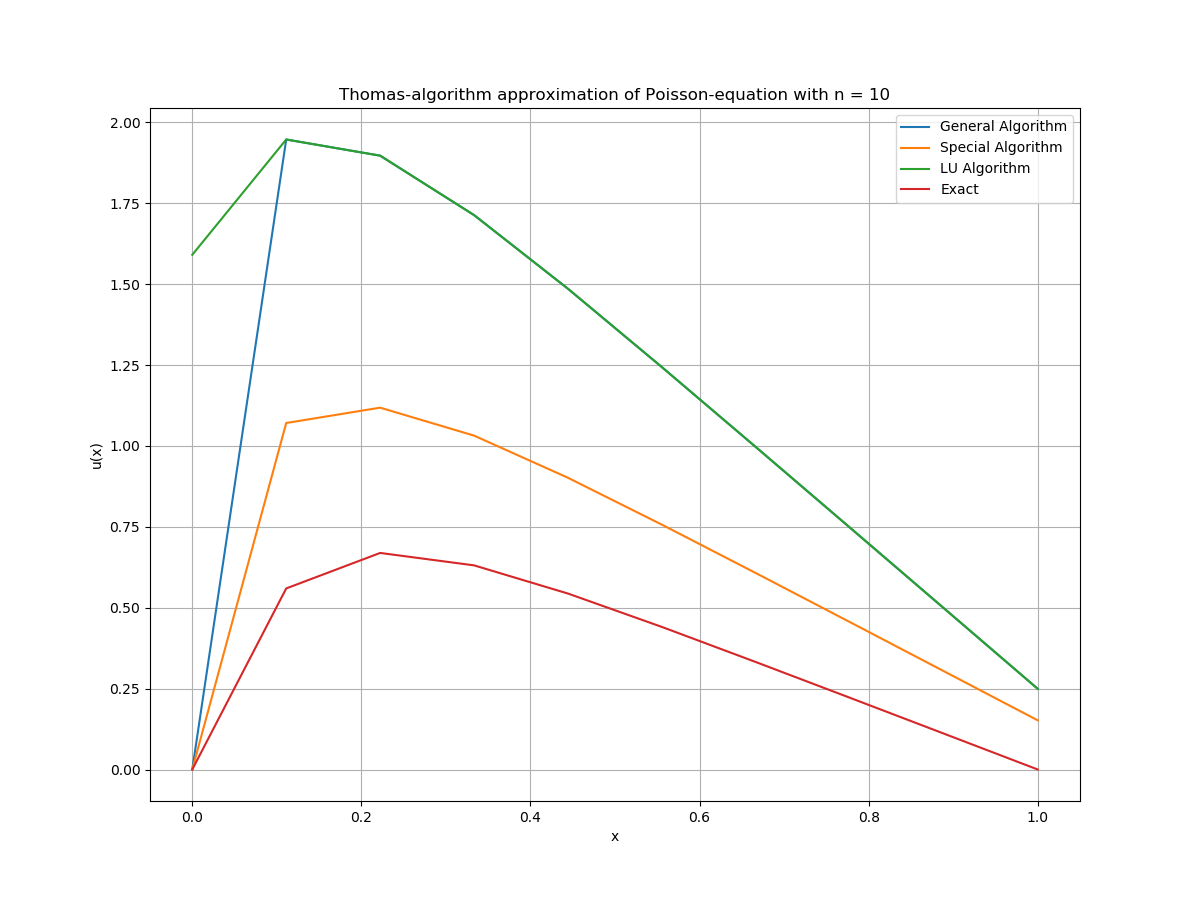
\includegraphics[width = 11cm]{program/data10.png}
	\caption{The plot of the different algorithm for $n = 10$. }
	\label{fig:data10png}
\end{figure}

\begin{figure}[ht]
	\centering
	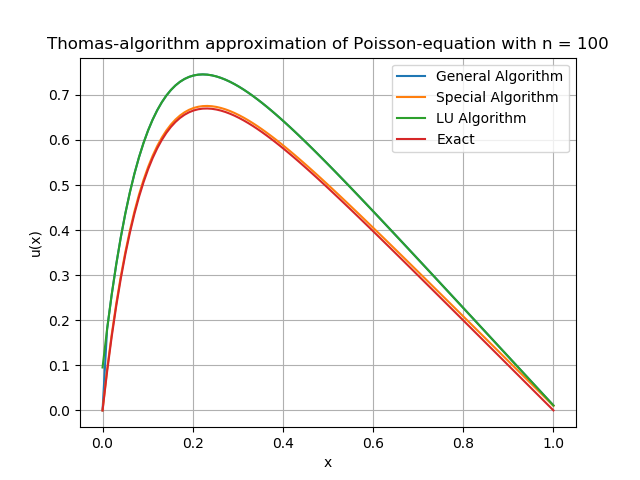
\includegraphics[width = 11cm]{program/data100.png}
	\caption{The plot of the different algorithm for $n = 100$. }
	\label{fig:data100png}
\end{figure}

\begin{figure}[ht]
	\centering
	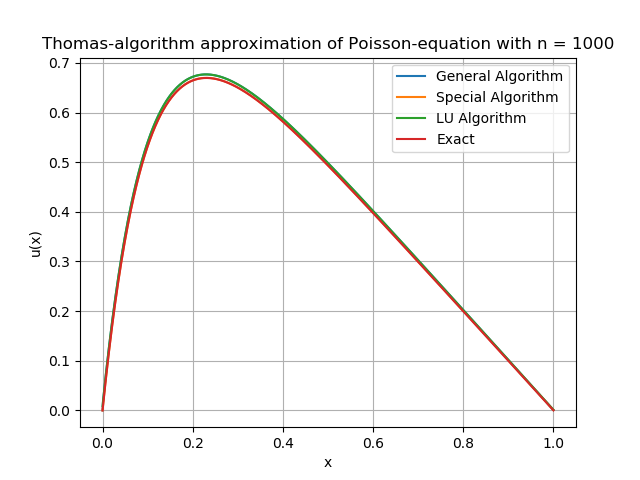
\includegraphics[width = 11cm]{program/data1000.png}
	\caption{The plot of the different algorithm for $n = 1000$. }
	\label{fig:data1000png}
\end{figure}



\clearpage

%----------------Refrences----------------------------------------
\vspace{1cm}

\section{Refrences}

\href{https://github.com/CompPhysics/ComputationalPhysics/blob/master/doc/Projects/2019/Project1/pdf/Project1.pdf}{Link to the PDF of the project}

\href{https://github.com/Erikbgram/Fys3150}{Link to our GitHub-repository}. \\

\href{http://www.industrial-maths.com/ms6021_thomas.pdf}{Link to an article about the tridiagonal matrix algorithm}. This includes general theory about the algorithm and how it works. \\

\href{https://github.com/CompPhysics/ComputationalPhysics/blob/master/doc/Lectures/lectures2015.pdf}{Link to lecture slides in FYS3150 - Computational Physics}. See page 168 and the rest of chapter \textbf{6.4 Linear Systemts} for theory behind the tridiagonal matrix algorithm.






%----------------Slutten av dokumentet---------------------------------------



\end{document}
